\section{CI Pipeline Implementation [Rahat Rafiq]}\label{sec:ci_pipeline_implementaiton}

Azure DevOps continuous integration pipeline is designed to have one or more agent jobs, a single job consists of one or more tasks. In this implementation of the CI pipeline, there will be one agent job that consists of seven tasks. This agent job will be executed on a Microsoft hosted VM that azure DevOps dynamically assigns for each pipeline build. Thus it is necessary to have tasks in the pipeline that installs all the required services for each cycle.

\subsection{Pipeline Configuration}
The agent jobs and tasks of a pipeline and all its necessary parameters can be defined in two different ways. The first option is to use a configuration script written in YAML. The YAML configuration file has a specific syntax defined by Microsoft. It has a steps section that includes separate tasks, task section in turn will contain all the variables, parameters, and commands necessary to execute that specific task. ~\ref{fig:ci_pipeline_yaml_configuration_example} When creating the pipeline from azure DevOps a user will be prompted to use a YAML configuration file. There is also the other option to configure the job and tasks manually from the UI of azure DevOps However for achieving a high degree of automation it is better to utilize the YAML script. Because it essentially creates the CI pipeline with just a click and it also facilitates convenient cloning of the pipeline. While creating the pipeline a developer must set a trigger and define a Microsoft hosted VM for continuous integration. Both the trigger branch and the VM definition (Windows server or Linux) can be easily defined in the YAML script. ~\ref{fig:ci_pipeline_yaml_configuration_example}


\begin{figure}
    \centering
    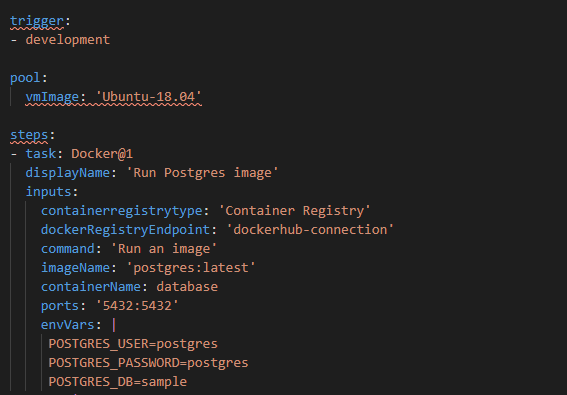
\includegraphics[width=10cm]{images/Rahat/ci_yaml.PNG}
    \caption{CI pipeline yaml configuration example}
    \label{fig:ci_pipeline_yaml_configuration_example}
\end{figure}



The following subsections discuss the tasks of the implemented CI pipeline solution of the spring boot application in detail:

\subsection{Get Source}
For each execution cycle, the CI pipeline will fetch the latest code-base from the specific branch of azure repos which triggered the build. 

\subsection{Postgresql Service Container}
Since the application properties of the application were edited to search for a PostgreSQL database server while building the application, it is mandatory to have a PostgreSQL server instance up and running in the machine before building the application. The most easiest and efficient way to install a PostgreSQL server on the hosted machine is to spin up a docker container. The hosted machine provided by azure DevOps where the CI pipeline is executing already comes with a pre-installed docker environment. The CI pipeline will just pull an official PostgreSQL image from the docker-hub registry with the help of a service connection and start up a PostgreSQL container and create a database inside the container. In the next task, the CI pipeline runs an azure CLI command to fetch the IP address of the running PostgreSQL container and update the spring data-source environment variable so the database container is available and ready to open connections to the application, which will start building in the next task of the pipeline. It is important to note that this PostgreSQL service container is only utilized as a test database while building and testing the application. It is not designed to serve as a production database. This test database container is destroyed at the end of every CI execution cycle.

\subsection{Build Gradle Application}
This task of the agent job essentially performs a gradlew build of the spring-boot application. However, while configuring the task it is important to define the SDK version that Gradle will use to build the solution. The SDK version defined in the Gradle build pipeline task should be the same as the SDK version that was used to develop the application. If the build is successful, a fat jar of the application will be created.

\subsection{Run Tests and Publish Results}
After building the application successfully, the CI pipeline will search for available test cases in the code-base. This task is designed to look for test cases in the src>test folder by default. It will perform all the Junit and integration test cases available in the test folder and publish the results of those tests in the azure test plans service. If a test case fails to pass the whole pipeline build will be canceled and an email notification will be sent to the DevOps organization members. CI pipeline also provides a detailed stack trace of the errors if the test case fails, which facilitates faster bug resolution.

\subsection{Package and Publish Artifacts}
The fat jar that was created from the build pipeline will be packaged and dropped to the azure artifacts directory. In this CI solution, some Kubernetes manifest files and ARM template and parameter files are also copied from the source azure repo and stored in the azure artifacts directory. This step of the job is performed because the continuous deployment pipeline can not directly access the source code repository in azure repos but it can access the artifacts directory.

\subsection{Build and Push Docker Image}
In the last step of the CI pipeline, the job will build the docker image of the spring boot application and push that image to a specific container registry. The docker image is built from a Dockerfile that is already available in the source code repository. Each image is tagged with the latest tag. This design decision was implemented to avoid pushing a new image each time the CI pipeline was executed, which might result in exceeding the storage limit of the container registry. The current solution is implemented to use an azure container registry with a basic SKU size (10GB). The spring boot application docker image consumes a fairly large disk space so the latest tag will overwrite the old image with the new one with each build and help save monetary resources. Finally, the pipeline will push the image to an azure container registry which is required to be created beforehand of the CI pipeline. A service connection is also needed to be established from the DevOps portal to the container registry for seamless image push events.